\documentclass[11pt]{article}            % Report class in 11 points
\parindent0pt  \parskip10pt             % make block paragraphs
\usepackage{graphicx}
\usepackage{listings}
\usepackage[document]{ragged2e}
\usepackage{float}
\newcommand\tab[1][1cm]{\hspace*{#1}}
\graphicspath{ {images/} }
\usepackage{graphicx} %  graphics header file
\begin{document}
\begin{titlepage}
    \centering
  \vfill
    
\includegraphics[width=8cm]{uni_logo.png} \\ 
	\vskip2cm
    {\bfseries\Large
	Data Structures  \& Algorithms \\ (CS09203)\\
	
	\vskip2cm
	Lab Report 
	 
	\vskip2cm
	}    

\begin{center}
\begin{tabular}{ l l  } 

Name: & Muhammad Umer \\ 
Registration \#: & CSU-F16-104 \\ 
Lab Report \#: & 11 \\ 
 Dated:& 25-06-2018\\ 
Submitted To:& Mr. Usman Ahmed\\ 

 %\hline
\end{tabular}
\end{center}
    \vfill
    The University of Lahore, Islamabad Campus\\
Department of Computer Science \& Information Technology
\end{titlepage}


    
    {\bfseries\Large
\centering
	Experiment \# 1 \\

Implement MST (Minimum Spanning Tree) on the given graph.\\
	
	}    
 \vskip1cm
 \textbf {Objective}\\  To understand and implement the Minimum Spanning Tree on the graph with different cycles.
 
 \textbf {Software Tool} \\
1. Sublime Text Editor\\
2. Dev C++\\
3. Window 7 (32 Bit)\\

\section{Theory }              
\justify Given a connected and undirected graph, a spanning tree of that graph is a subgraph that is a tree and connects all the vertices together. A single graph can have many different spanning trees. A minimum spanning tree (MST) or minimum weight spanning tree for a weighted, connected and undirected graph is a spanning tree with weight less than or equal to the weight of every other spanning tree. The weight of a spanning tree is the sum of weights given to each edge of the spanning tree.\\~\\ A minimum spanning tree has (V – 1) edges where V is the number of vertices in the given graph.\\~\\
\subsection{Procedure: Task 1 Implement MST on graph}
Implement the MST Minimum Spanning Tree on the following graph:
\begin{figure}[H]
\centering
  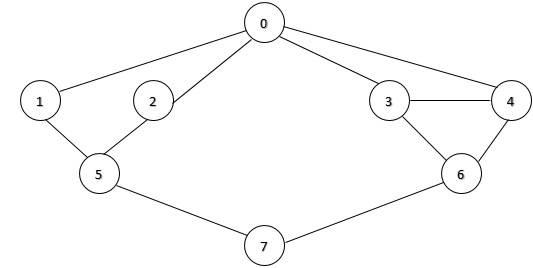
\includegraphics[width=12cm,height=6cm,keepaspectratio]{graph.png}    
\end{figure}
\begin{lstlisting}[language=C++]
#include <stdio.h>
#include <stdlib.h>
#include <string.h>

struct Edge
{
    int src, dest, weight;
};
struct Graph
{
    int V, E;
    struct Edge* edge;
};
 
// Creates a graph with V vertices and E edges
struct Graph* createGraph(int V, int E)
{
    struct Graph* graph = new Graph;
    graph->V = V;
    graph->E = E;
 
    graph->edge = new Edge[E];
 
    return graph;
}
struct subset
{
    int parent;
    int rank;
};
int find(struct subset subsets[], int i)
{
    if (subsets[i].parent != i)
        subsets[i].parent = find(subsets, subsets[i].parent);
 
    return subsets[i].parent;
}
void Union(struct subset subsets[], int x, int y)
{
    int xroot = find(subsets, x);
    int yroot = find(subsets, y);
    if (subsets[xroot].rank < subsets[yroot].rank)
        subsets[xroot].parent = yroot;
    else if (subsets[xroot].rank > subsets[yroot].rank)
        subsets[yroot].parent = xroot;
    else
    {
        subsets[yroot].parent = xroot;
        subsets[xroot].rank++;
    }
}
// Compare two edges according to their weights.
// Used in qsort() for sorting an array of edges
int myComp(const void* a, const void* b)
{
    struct Edge* a1 = (struct Edge*)a;
    struct Edge* b1 = (struct Edge*)b;
    return a1->weight > b1->weight;
}
// The main function to construct MST using Kruskal's algorithm
void KruskalMST(struct Graph* graph)
{
    int V = graph->V;
    struct Edge result[V];  // Tnis will store the resultant MST
    int e = 0;  // An index variable, used for result[]
    int i = 0;  // An index variable, used for sorted edges
    qsort(graph->edge, graph->E, sizeof(graph->edge[0]), myComp);
    struct subset *subsets = (struct subset*) malloc( V * sizeof(struct subset) );
    for (int v = 0; v < V; ++v)
    {
        subsets[v].parent = v;
        subsets[v].rank = 0;
    }
    while (e < V - 1)
    {
        struct Edge next_edge = graph->edge[i++];
        int x = find(subsets, next_edge.src);
        int y = find(subsets, next_edge.dest);
        if (x != y)
        {
            result[e++] = next_edge;
            Union(subsets, x, y);
        }
    }
    // built MST
    printf("Following are the edges in the constructed MST\n");
    for (i = 0; i < e; ++i)
        printf("%d -- %d == %d\n", result[i].src, result[i].dest, result[i].weight);
    return;
}
int main()
{
    int V = 4;  // Number of vertices in graph
    int E = 5;  // Number of edges in graph
    struct Graph* graph = createGraph(V, E);
    // add edge 0-1
    graph->edge[0].src = 0;
    graph->edge[0].dest = 1;
    graph->edge[0].weight = 10;
    // add edge 0-2
    graph->edge[1].src = 0;
    graph->edge[1].dest = 2;
    graph->edge[1].weight = 6;
    // add edge 0-3
    graph->edge[2].src = 0;
    graph->edge[2].dest = 3;
    graph->edge[2].weight = 5;
    // add edge 1-3
    graph->edge[3].src = 1;
    graph->edge[3].dest = 3;
    graph->edge[3].weight = 15;
    // add edge 2-3
    graph->edge[4].src = 2;
    graph->edge[4].dest = 3;
    graph->edge[4].weight = 4;
    KruskalMST(graph);
    return 0;
}
\end{lstlisting}
 \textbf Output: Consider the Figure 1 for the output of the above code in the end of this document.

\textbf{Source Code} \\
https://goo.gl/ccBvqK

\begin{figure}[b!]
\centering
  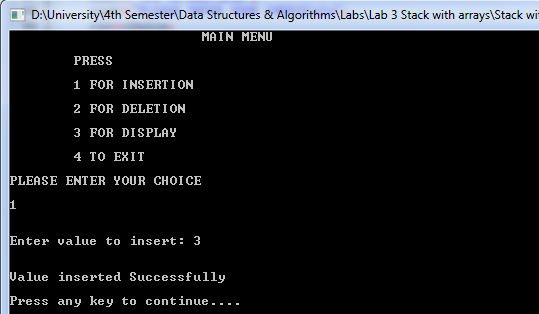
\includegraphics[width=12cm,height=6cm,keepaspectratio]{1.png}
\caption{Minimum Spanning Tree implementation on graph}
\label{Figure:1}    
\end{figure}

\section{Conclusion}
\justify Graphs are used to represent many real life applications: Graphs are used to represent networks. The networks may include paths in a city or telephone network or circuit network. Minimum Spanning Tree algorithm can be implemented on graphs to visit every node in the shortest path, graphs may contain cycles, so we may come to the same node again. To avoid processing a node more than once, we use a boolean visited array.\\~\\

\tab[6cm] \noindent\rule{6cm}{0.4pt}\\
\tab[6cm] (Concerned Teacher/Lab Engineer)


 
\end{document}                          % The required last line
